
\section*{CHƯƠNG 1. HƯỚNG DẪN CÀI ĐẶT}
\setcounter{section}{1}
\setcounter{subsection}{0} %LƯU Ý MỖI LẦN THÊM CHƯƠNG MỚI CẦN THÊM CÂU NÀY ĐỂ RESET THỨ TỰ CỦA SUBSECTON VỀ 1
\setcounter{table}{0} % LƯU Ý SAU MỖI LẦN GỌI BẢNG HAY HÌNH ẢNH PHẢI THÊM CÂU NÀY ĐỂ RESET THỨ TỰ
\setcounter{figure}{0} %% LƯU Ý SAU MỖI LẦN GỌI BẢNG HAY HÌNH ẢNH PHẢI THÊM CÂU NÀY ĐỂ RESET THỨ TỰ
\addcontentsline{toc}{section}{\numberline{}CHƯƠNG 1. HƯỚNG DẪN CÀI ĐẶT}
\textbf{WazNet} là ứng dụng đã có mặt trên cả hai nền tảng Android và iOS. Để cài đặt người dùng có thể truy cập vào cửa hàng ứng dụng theo hệ điều hành và tìm kiếm \textbf{WazNet} để tải về và cài đặt. Hoặc có thể truy cập vào link dưới đây:
\begin{adjustwidth}{1.5em}{}
  \begin{itemize}
    \item Link cài đặt ứng dụng trên \href{https://play.google.com/store/apps/details?id=vn.sparc.waznet}{Android}
    \item Link cài đặt ứng dụng trên \href{https://apps.apple.com/vn/app/waznet/id6738925384}{iOS}
  \end{itemize}
\end{adjustwidth}

% \begin{figure}[H]
%   \centering
%   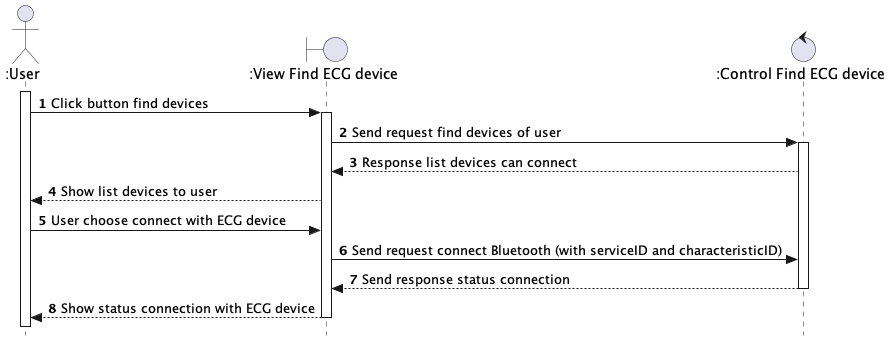
\includegraphics[width=14cm,height=6cm]{Images/mobile_app/connect_with_device.png}
%   \caption[Hình ảnh ứng dụng trên Store]{\bfseries \fontsize{12pt}{0pt}
%   \selectfont Hình ảnh ứng dụng trên Play Store (Android)}
%   \label{ios_store_app} %đặt tên cho ảnh
% \end{figure}

% \begin{figure}[H]
%   \centering
%   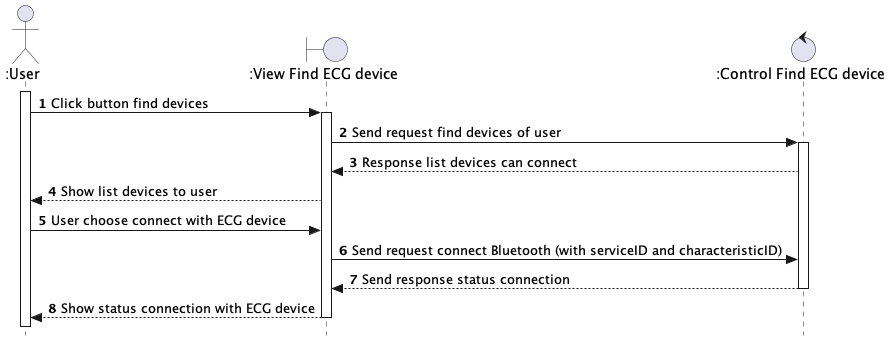
\includegraphics[width=14cm,height=6cm]{Images/mobile_app/connect_with_device.png}
%   \caption[Hình ảnh ứng dụng trên Store]{\bfseries \fontsize{12pt}{0pt}
%   \selectfont Hình ảnh ứng dụng trên App Store (iOS)}
%   \label{ios_store_app} %đặt tên cho ảnh
% \end{figure}

\newpage
